\pdfoutput=1
\documentclass[12pt,a4paper]{report}
\usepackage[a4paper,left=32mm,right=25mm,top=27mm,bottom=27mm]{geometry}
\usepackage[pdftex]{graphicx}
\usepackage{array}
\usepackage{longtable}
\usepackage{url}
\renewcommand{\baselinestretch}{1.4}
\setlength{\parindent}{1.2em}
\setlength{\parskip}{0.25em}
\setlength{\emergencystretch}{2em}
\graphicspath{{figures/}{../bench/dp_fib/figures/}}

\newcommand{\projecttitle}{A Domain-Specific Programming Language and Compiler for Competitive Programming}
\newcommand{\vulp}{\textsc{Vulp}}
\renewcommand{\bibname}{References}

\begin{document}
\begin{titlepage}
\renewcommand{\baselinestretch}{1}\normalsize
\centering
\vspace*{0.1cm}
{\Large\bfseries\MakeUppercase{\projecttitle}\par}
\vspace{1.2cm}
{A Project Report Submitted\\
in Partial Fulfilment of the Requirements\\
for the Degree of\par}
\vspace{0.5cm}
{\Large\bfseries Bachelor of Technology\par}
\vspace{0.5cm}
{Phase 1, Review 2\\Group 14\par}
\vspace{0.5cm}
{\itshape by\par}
\vspace{0.3cm}
{\large\bfseries
Vibhaas Nirantar Srivastava (2023BCS0037)\\
Harsh Kumar (2023BCS0133)\\
Malampati Charan (2023BCS0217)\\
Aysha Lintha (2023BCS0183)\par}
\vspace{0.5cm}
Under the Supervision of\\[4pt]
{\large\bfseries Dr. P. Victer Paul}\par
\vfill

\includegraphics[width=3.3cm]{logo2.jpg}\par
\vspace{0.4cm}
{\bfseries DEPARTMENT OF COMPUTER SCIENCE AND ENGINEERING\\
INDIAN INSTITUTE OF INFORMATION TECHNOLOGY\\
KOTTAYAM-686635, INDIA\par}
\vspace{0.35cm}
October 2026
\end{titlepage}
\renewcommand{\baselinestretch}{1.4}\normalsize

\pagenumbering{roman}
\setcounter{page}{2}
\chapter*{Declaration}
\addcontentsline{toc}{chapter}{Declaration}
We, the four members of Group 14 named on the title page, declare that the project report entitled ``\projecttitle'' records our work on the \vulp{} language and compiler for the Phase 1 Review 2 submission. Material drawn from other work is acknowledged in the text and references. This report has not been submitted for the award of another degree or diploma.

\vspace{2.5cm}
\noindent Kottayam-686635\hfill \rule{6.2cm}{0.4pt}\\
October 2026\hfill Group 14 signatures
\clearpage

\chapter*{Certificate}
\addcontentsline{toc}{chapter}{Certificate}
This is to certify that the project report entitled ``\projecttitle'' is submitted by Vibhaas Nirantar Srivastava (2023BCS0037), Harsh Kumar (2023BCS0133), Malampati Charan (2023BCS0217), and Aysha Lintha (2023BCS0183) towards the requirements for the Bachelor of Technology degree at the Indian Institute of Information Technology Kottayam under the supervision of Dr. P. Victer Paul. The certificate is to be signed by the project supervisor after review.

\vspace{3cm}
\noindent Kottayam-686635\hfill \rule{6.2cm}{0.4pt}\\
October 2026\hfill Dr. P. Victer Paul, Project Supervisor
\clearpage

\chapter*{Abstract}
\addcontentsline{toc}{chapter}{Abstract}
Contest programs often repeat the same work around an algorithm: reading input, handling several testcases, and setting up a suitable data structure. We built \vulp{}, a statically typed language and LLVM-based compiler, to make some of that work part of the language. Its first version includes a lexer, a Pratt parser, semantic checks, LLVM IR generation, native compilation, and an in-process JIT. Programs can use buffered input, testcase blocks, integers up to 256 bits, arrays, vectors, maps, structures, and range-declared integers. The \texttt{dp fn} construct memoizes eligible recursive functions. Before generating a cache, the compiler checks for side effects; a function that reads global data has its cache reset between testcases.

We compared six \vulp{} programs with C++ and Python programs on the reference laptop. Five use fewer source tokens than the C++ versions. Dijkstra is the exception because we had to write a heap in \vulp{}. Four programs run within 17\% of the C++ time. Map counting takes 1.42 times as long. For longest common subsequence, the 32-bit tables take 0.033 s in \vulp{} and 0.024 s in C++. We also compared \texttt{dp fn} with direct, unmemoized Fibonacci recursion. At \texttt{fib(40)}, the median time is 1.57 ms for \texttt{dp fn}, 198 ms for plain \vulp{}, 107 ms for plain C++, and 8.26 s for plain Python. A dense table remains preferable for some dynamic programs, as the LCS results show.

The proposal extends beyond this compiler version. Selection of range-query structures and graph layouts, modular arithmetic types, complexity annotations, and a possible small language model are still planned. The report describes the current implementation, its tests and measurements, and the work left for the next phase.
\clearpage

\chapter*{Acknowledgment}
\addcontentsline{toc}{chapter}{Acknowledgment}
We thank our supervisor, Dr. P. Victer Paul, for his guidance on this project. We also thank the Department of Computer Science and Engineering at IIIT Kottayam for the opportunity to carry out the work and the project review panel for its feedback on the scope and evaluation.
\clearpage

\tableofcontents
\clearpage
\listoffigures
\clearpage
\listoftables
\clearpage
\pagenumbering{arabic}

\chapter{Introduction}
\section{Background and motivation}
\subsection{What competitive programming involves}
In a programming contest, participants write programs to solve algorithmic problems within a fixed time. Each problem specifies the input, the required output, and limits on the input size. The source program is submitted to an online judge, which runs it on test inputs that the participant may not see. The judge accepts the program only when the output is correct and the run stays within its time and memory limits. We call the submitted program a \emph{contest program}. A \emph{testcase} is one independent instance of the problem.

For example, a problem may supply several arrays and ask for the largest sum of a contiguous part of each one. A submitted program has to read the number of arrays, read each array, calculate its answer, and print the answers in the specified format. The calculation itself needs only a running sum. Reading the input and managing the testcases take additional code, and an error there can cause the judge to reject an otherwise correct algorithm.

Constraints also determine how a program stores data. An adjacency matrix for a graph with a hundred thousand vertices would be impractical, so a contestant will normally use adjacency lists. For a dynamic program with millions of states, the choice between 32-bit and 64-bit table elements may determine whether it fits in memory. A rolling-row table can reduce memory further when the recurrence permits it. These are routine decisions made while the contest clock is running.

\subsection{Why a language can help}
C++ is widely used in contests for its native speed and algorithm libraries. Contestants still have to assemble input handling and data structures for each submission. Python programs can be shorter, but some loops and large collections are costly under a strict limit. We wanted a small language that would make common contest work easier to express and still produce a native executable.

The first version of \vulp{} addresses three recurring pieces of code. \texttt{TC:} repeats a block for each testcase, \texttt{read} handles token input, and \texttt{dp fn} adds checked memoization to a recursive function. The language also lets a programmer choose integer widths and use several containers. Our proposal describes a broader CPIR design that would retain information about range queries, graph mutability, and dynamic-programming dependencies. That representation and its selection passes have yet to be implemented.

\section{Problem statement and objectives}
Our project is to design a language and compiler for competitive programming, with our own lexer and parser and an LLVM IR backend. The proposed language includes graphs, bitsets, Fenwick trees, segment trees, modular arithmetic types, range-bounded variables, and time and memory complexity annotations. We may also study a small language model for estimating complexity when static analysis cannot prove a bound. The full evaluation is planned against C, C++, Java, and Python, using writing effort, source size, execution time, and memory as separate measures.

For this review, the working objectives are:
\begin{itemize}
\item define a small language with predictable types, control flow, ownership, and errors;
\item compile representative contest programs through LLVM and validate their output;
\item measure source size, execution time, and memory against equivalent C++ and Python programs; and
\item identify which goals from the original proposal require new language or compiler work.
\end{itemize}

\section{Scope of this review}
The compiler now supports scalar types, arrays, vectors, ordered maps, structures, functions, loops, buffered input, and \texttt{dp fn}. It emits LLVM IR for either JIT execution or a native executable. We have measured six tasks against C++ and Python, along with memoized and plain Fibonacci recursion. The C and Java baselines, a study of programmer time, and the proposed set of 40 to 50 problems remain for later reviews. Chapter~\ref{ch:progress} lists the status of each proposal item.

\chapter{Related work and design context}
The AtCoder Library provides contest data structures including Fenwick trees and segment trees~\cite{atcoder}. KACTL collects short, tested C++ algorithms intended for contest use~\cite{kactl}. Both resources reduce the need to derive an implementation during a contest. They also motivate the proposed \vulp{} abstractions: if a source program states the operations and algebraic properties, a later compiler pass could select the representation. This selection is part of our proposal and has not been implemented in V1.

LLVM provides the intermediate representation, optimization passes, JIT infrastructure, and object-code generation used by \texttt{vulpc}. Its integer type permits explicit widths, which makes it a suitable backend for \vulp{}'s integer types~\cite{llvmref}. The LLVM frontend tutorial describes a lexer, parser, abstract syntax tree, and code-generation path similar to the broad shape of our pipeline~\cite{llvmtutorial}. \vulp{} adds its own type rules, container semantics, runtime library, and contest constructs on top of that path.

GraphIt demonstrates how a domain-specific graph representation can retain information useful for choosing a schedule and generated implementation~\cite{graphit}. That result informs the proposed graph and range-query features, although our present compiler does not carry a graph-specific IR. Work on comparative programming-language evaluation also supports measuring code size and runtime on matching tasks instead of arguing from syntax examples alone~\cite{nanz}. Resource-analysis research shows ways to prove useful bounds for restricted programs~\cite{knoth}. It does not justify claiming that arbitrary program complexity can be inferred. For the proposed complexity annotation feature, a result must be reported as verified, unresolved, or unsupported by the analysis being used.

\chapter{System design}\label{sec:system}
\section{Compiler pipeline}
Figure~\ref{fig:pipeline} shows the path from a \texttt{.vp} file to a running program. The lexer records the position of each token for error messages. A Pratt parser turns the tokens into an abstract syntax tree. Semantic analysis then resolves names and types, checks calls and control flow, and applies the rules for \texttt{dp fn} and reference parameters. Code generation produces LLVM IR. Finally, the driver runs LLVM optimization and either executes the module through ORC JIT or links a native executable from an object file.

\begin{figure}[htbp]
\centering
\setlength{\fboxsep}{8pt}
\fbox{\begin{minipage}{0.88\textwidth}\centering
\texttt{.vp source} $\longrightarrow$ lexer $\longrightarrow$ parser $\longrightarrow$ semantic analysis\\[7pt]
$\longrightarrow$ LLVM IR generation $\longrightarrow$ LLVM optimization\\[7pt]
$\longrightarrow$ ORC JIT \quad or \quad object file and native linker
\end{minipage}}
\caption{The \vulp{} compilation pipeline.}
\label{fig:pipeline}
\end{figure}

\section{Language constructs}
\subsection{Program structure and a complete example}
A \vulp{} source file ends in \texttt{.vp}. Top-level statements run in source order; there is no separate \texttt{main} function. Functions and structures are also defined at the top level, and functions may be called before their definitions. Statements end with semicolons. Braces make a block and introduce a local scope. An uninitialized variable starts with the zero or empty value of its type.

The program below solves the maximum contiguous subarray sum problem from Chapter~1. Its input begins with the number of testcases. On each iteration, \texttt{TC:} executes the block again, \texttt{read int[n] a} allocates and fills an array, and \texttt{println} writes the answer.
\begin{verbatim}
TC: {
    read int n;
    read int[n] a;
    int best = a[0], current = 0;
    for x in a: {
        current = max(current + x, x);
        best = max(best, current);
    }
    println(best);
}
\end{verbatim}
The loop visits each element once. The program assumes $n>0$, which the problem statement would have to guarantee. In \texttt{for x in a}, \texttt{x} receives a copy of the element. Assigning to \texttt{x} would leave the array unchanged.

Running \texttt{vulpc solution.vp} executes the file through the JIT. The command \texttt{vulpc solution.vp -o solution} produces a native executable that can be given the judge's input. Both modes follow the same language rules and use the same runtime library. We used native executables for the runtime comparison.

\subsection{Types and integer representation}
Table~\ref{tab:types} lists the principal built-in types. An array dimension is evaluated when its declaration runs. For example, \texttt{int[n][m] grid;} makes $n$ rows of $m$ zero-initialized integers. The array length then stays fixed. A vector can grow through \texttt{push}.

\begin{table}[htbp]
\centering\small
\begin{tabular}{|>{\raggedright\arraybackslash}p{32mm}|>{\raggedright\arraybackslash}p{47mm}|>{\raggedright\arraybackslash}p{60mm}|}
\hline
Type form & Meaning & Example use\\\hline
\texttt{int}, \texttt{iN}, \texttt{uN} & Signed 64-bit integer; explicit signed or unsigned width up to 256 bits & \texttt{i32 count;} for a compact table element\\\hline
\texttt{int<lo..hi>} & Chooses the smallest supported signed storage width that fits both bounds & \texttt{int<0..1000000007> x;} uses 32-bit storage\\\hline
\texttt{bool}, \texttt{char}, \texttt{float} & Logical value, byte character, and 64-bit floating-point value & \texttt{bool seen = false;}\\\hline
\texttt{string}, \texttt{T[n]}, \texttt{vec<T>} & Byte string, fixed-length array, and growable sequence & \texttt{vec<int>[n] adj;} for adjacency lists\\\hline
\texttt{map<K,V>}, \texttt{struct} & Ordered key-value map and named record with fields & \texttt{map<string,int> freq;}\\\hline
\end{tabular}
\caption{The main \vulp{} type forms and their intended use.}
\label{tab:types}
\end{table}

\noindent\begin{minipage}{\linewidth}
Integer widths round up to one of 8, 16, 32, 64, 128, or 256 bits. Thus \texttt{i21} occupies 32 bits. So does \texttt{int<0..1000000007>}. Arithmetic first promotes values narrower than 64 bits to \texttt{int}, and an assignment back to a narrow variable may truncate the result. A range declaration chooses the storage width; V1 does not enforce the declared interval on every later assignment. The compiler rejects an out-of-range constant, and the runtime rejects input that does not fit the storage type. A range declaration therefore does not establish a permanent bound on the variable's value.
\end{minipage}

\subsection{Control flow and structured input}
An \texttt{if}, \texttt{while}, or \texttt{for} condition must be a \texttt{bool}. For instance, \texttt{if n \% 2 == 1:} is valid, while an integer used directly as the condition is a type error. A colon follows the control-flow header, then a statement or block. The language has C-style loops and \texttt{for x in} loops. The latter can traverse arrays, vectors, strings, ordered-map keys, and inclusive ranges such as \texttt{[1..n]}. For a range, the compiler uses a counter rather than allocating an array.

The buffered reader treats whitespace as a token separator. \texttt{read int n;} declares and reads one integer. After $n$ is known, \texttt{read int[n] a;} allocates the array and reads its elements. \texttt{read(x, a[i]);} writes into existing locations instead. \texttt{print} writes its arguments without separators, and \texttt{println} adds a newline. Arrays and vectors are printed with spaces between elements. Before the runtime waits for more input, it flushes pending output so that an interactive judge can receive it.

\texttt{TC:} reads a count and executes its block once per testcase. Local variables are initialized again on each iteration. Inside the block, \texttt{continue} starts the next testcase and \texttt{break} ends the repetition. \texttt{TC:} cannot be nested or used inside a function.

\subsection{Containers, structures, and ownership}
Arrays have indexing, length, and sorting operations. Their length cannot change. Vectors add \texttt{push}, \texttt{pop}, and \texttt{clear}, while strings are mutable byte sequences. Map keys are ordered, so iteration returns them in sorted order. Reading a missing key yields the value type's zero value without inserting an entry. Writing through a map index does insert one. A structure can hold, for example, the destination and weight of a graph edge:
\begin{verbatim}
struct Edge { int to; i32 weight; }
vec<Edge>[n + 1] adj;
adj[u].push(Edge(v, w));
\end{verbatim}
This adjacency list is built by the programmer. V1 has no built-in graph type and does not choose between adjacency vectors and compressed sparse rows.

Containers have value semantics. With \texttt{vec<int> b = a;}, \texttt{b} receives a deep copy, and \texttt{b.push(3)} leaves \texttt{a} alone. Function arguments are copied too unless the parameter type ends in \texttt{\&}. A reference parameter can update the caller's value or avoid copying a large container. Resizing a container may invalidate a reference to an element, so semantic analysis rejects calls that could leave such a reference dangling. Heap-owning values are released on overwrite or at the end of their scope; temporaries are released after use.

\subsection{Functions and calls}
A function starts with \texttt{fn} and typed parameters. A return type follows \texttt{->}; a procedure with no return value omits it. Recursive calls are allowed. For a function that returns a value, the compiler checks that every reachable path returns. Here is a greatest common divisor function:
\begin{verbatim}
fn gcd(int a, int b) -> int {
    while b != 0: {
        int old = b;
        b = a % b;
        a = old;
    }
    return a;
}
\end{verbatim}
Arguments are evaluated from left to right. An ordinary parameter receives a value, including a deep copy when the argument is a container. A \texttt{T\&} parameter refers to the caller's variable, element, or field and requires an exact type match. The compiler checks for reference hazards before code generation. Built-ins such as \texttt{min}, \texttt{max}, and \texttt{abs} use the same call syntax as other functions.

\section{Memoized functions}
Memoization requires one extra keyword in the function declaration:
\begin{verbatim}
dp fn fib(int n) -> int {
    if n <= 1: return n;
    return fib(n - 1) + fib(n - 2);
}
\end{verbatim}
For an eligible \texttt{dp fn}, the compiler generates the function body and a wrapper. Every call goes through that wrapper, including calls made by the function itself. The wrapper looks up the argument values in a runtime hash table. If the result is present, it returns the stored value. Otherwise it runs the body and stores the answer. In Fibonacci recursion, the same value of $n$ appears on many branches; the body runs only once for each distinct value reached.

The compiler applies the following restrictions before it generates the cache:
\begin{itemize}
\item Parameters must be integers, characters, or booleans, and the result must be a scalar. This gives the cache a fixed-size key and value.
\item The function must not write a global or perform input/output, directly or through a function it calls. A repeated call must not skip an observable side effect.
\item Reading globals is allowed. If a \texttt{dp fn} reads global state, its cache is reset before each \texttt{TC:} iteration so that one testcase cannot reuse an answer computed from another testcase's data.
\end{itemize}
Generation tags let the runtime reset a memo table in constant time without clearing each occupied slot. A function that reads no globals keeps its cache throughout the program. A programmer who changes a global dependency outside \texttt{TC:} must account for a cache that has not been reset. Each state also costs a hash lookup and storage space. A dense array may therefore run faster for a regular dynamic program; Section~\ref{sec:evaluation} includes an example.

\section{Runtime and diagnostics}
The runtime library implements buffered input and output, containers, integer conversion, and memo tables. The JIT calls it inside the compiler process; native executables link the static runtime library. Compile errors show the source line with a caret at the error. Checked runtime operations also identify the relevant line when they encounter:
\begin{itemize}
\item an array, vector, or string index outside its valid range;
\item division by zero or removal from an empty container; and
\item exhausted input or an input integer that does not fit its target type.
\end{itemize}
With \texttt{--no-checks}, the compiler omits its generated bounds and division checks. The implementation uses LLVM 18 and C++20.

\chapter{Implementation and validation}
\section{Implemented components}
The source program passes through the components listed in Table~\ref{tab:components}. Each frontend stage reports the errors it finds. The parser builds expressions by precedence and recovers from some statement errors, allowing one compilation to report more than one mistake. Semantic analysis interns types, resolves scopes, checks operators and calls, determines which functions are safe to memoize, and checks reference hazards.

\begin{table}[htbp]
\centering\small
\begin{tabular}{|>{\raggedright\arraybackslash}p{32mm}|>{\raggedright\arraybackslash}p{107mm}|}
\hline
Component & Work performed\\\hline
Lexer & Converts source bytes into tokens with line and column locations; recognizes literals, identifiers, keywords, and operators.\\\hline
Parser & Constructs statements, expressions, function definitions, structures, and type syntax using a Pratt expression parser.\\\hline
Semantic analysis & Resolves names and types; checks returns, control flow, reference safety, and transitive side effects of \texttt{dp fn}.\\\hline
LLVM code generation & Emits arithmetic and control-flow operations, runtime calls, container helpers, and memoization wrappers; verifies the resulting module.\\\hline
Driver and runtime & Runs optimized IR through ORC JIT or emits and links an object file; supplies buffered I/O, containers, and memo tables.\\\hline
\end{tabular}
\caption{Responsibilities of the implemented compiler and runtime stages.}
\label{tab:components}
\end{table}

The typed syntax tree currently lowers straight to LLVM IR. The proposal describes a separate CP semantic IR for range-query operations, dynamic-programming dependencies, and graph mutability. Those planned passes need to see operations before they are lowered into a particular data structure. The current frontend and execution path provide a starting point for that work.

\section{Tests and review}
We tested the compiler stages separately and ran generated programs. There are 142 unit tests, 34 end-to-end programs run in three modes, 20 programs that should fail compilation, and 10 examples. Another 88 runs under AddressSanitizer produced no report. The end-to-end runner compares expected output in JIT and native modes. Table~\ref{tab:validation} gives the purpose of each test group.

\begin{table}[htbp]
\centering\small
\begin{tabular}{|>{\raggedright\arraybackslash}p{39mm}|r|>{\raggedright\arraybackslash}p{89mm}|}
\hline
Check & Count & Purpose\\\hline
Unit tests & 142 & Lexer, parser, types, semantic rules, runtime operations, and code generation.\\\hline
End-to-end programs & 34 & Expected output under JIT, native execution, and a mode that poisons freed memory.\\\hline
Expected compile errors & 20 & Diagnostic category, message, and nonzero exit status for invalid programs.\\\hline
Examples & 10 & Short programs demonstrating language features with expected output.\\\hline
AddressSanitizer runs & 88 & Memory-error checks on generated programs and the runtime at two optimization levels.\\\hline
\end{tabular}
\caption{Validation performed for the first compiler version.}
\label{tab:validation}
\end{table}

Review and testing found faults in container ownership, integer corner cases, reference-parameter aliasing, and expression evaluation order. We fixed them and added regression programs. The test results support the behavior described here, though they cannot prove correctness for every program a contestant might write.

\chapter{Evaluation}\label{sec:evaluation}
\section{Method and workloads}
We ran six task families on a Linux laptop with an AMD Ryzen 9 8940HX processor. The \vulp{} compiler used LLVM 18.1.3. C++ programs were built with GCC 13.3 and \texttt{-O2 -std=c++20}; the Python version was CPython 3.12.3. For each task, a fixed seed generated one input used by all three implementations. The harness checked SHA-256 hashes of the complete outputs before it accepted any timing. It then ran the programs in seven interleaved rounds on one pinned CPU. The figures report median wall time and median peak resident memory. We measured build time separately over three builds and counted source tokens after removing comments and blank lines.

The Python 3 harness obtained the measurements as follows:
\begin{itemize}
\item \textbf{Elapsed time:} the \texttt{perf\_counter()} clock from Python's \texttt{time} module brackets each process run. This wall time includes process startup and the timing wrapper. The same clock brackets compiler invocations for separate build-time measurements.
\item \textbf{Peak memory:} GNU \texttt{/usr/bin/time} runs each program. Its \texttt{\%M} field gives the maximum resident set size in KiB; the harness divides by 1024 to report MiB. The value includes the whole process, including the Python interpreter when relevant.
\item \textbf{CPU placement:} \texttt{taskset -c 7} pins the timed runs to the same CPU. The runtime comparison uses prebuilt native \vulp{} and C++ executables and a Python script.
\end{itemize}

The six tasks put different demands on the language:
\begin{itemize}
\item sieve counts primes to $2\times10^7$, stressing a tight array loop;
\item sort and I/O reads, sorts, and prints one million integers;
\item longest common subsequence (LCS) fills a table for two 3000-character strings;
\item Dijkstra uses a graph with $10^5$ vertices and $5\times10^5$ weighted edges;
\item the testcase task processes $2\times10^5$ small arrays; and
\item map counting performs one million insertions or updates.
\end{itemize}
The measurements cover execution and source size. They do not tell us how long a participant would need to learn \vulp{} or write one of the programs.

\section{Execution time and memory}
Table~\ref{tab:existing-time} gives the median times, with the same data plotted in Figure~\ref{fig:laptop-runtime}. The final column is \vulp{} time divided by C++ time; values below 1 mean that \vulp{} was faster in that run. For LCS, both compiled programs use bottom-up tables of 32-bit integers. The \vulp{} program has its normal runtime checks enabled.

\begin{table}[htbp]
\centering\small
\begin{tabular}{|>{\raggedright\arraybackslash}p{42mm}|r|r|r|r|}
\hline
Task & Vulp (s) & C++ (s) & Python (s) & Vulp/C++\\\hline
Sieve & 0.041 & 0.035 & 0.532 & 1.17\\\hline
Sort and I/O & 0.100 & 0.111 & 0.456 & 0.90\\\hline
LCS, i32 table & 0.033 & 0.024 & 0.645 & 1.37\\\hline
Dijkstra & 0.083 & 0.086 & 0.628 & 0.96\\\hline
Testcases & 0.055 & 0.055 & 0.305 & 0.99\\\hline
Map count & 0.275 & 0.194 & 0.275 & 1.42\\\hline
\end{tabular}
\caption{Median running times in seconds on the reference laptop. Lower is better. The LCS row uses 32-bit table elements in both compiled languages.}
\label{tab:existing-time}
\end{table}

\begin{figure}[htbp]
\centering
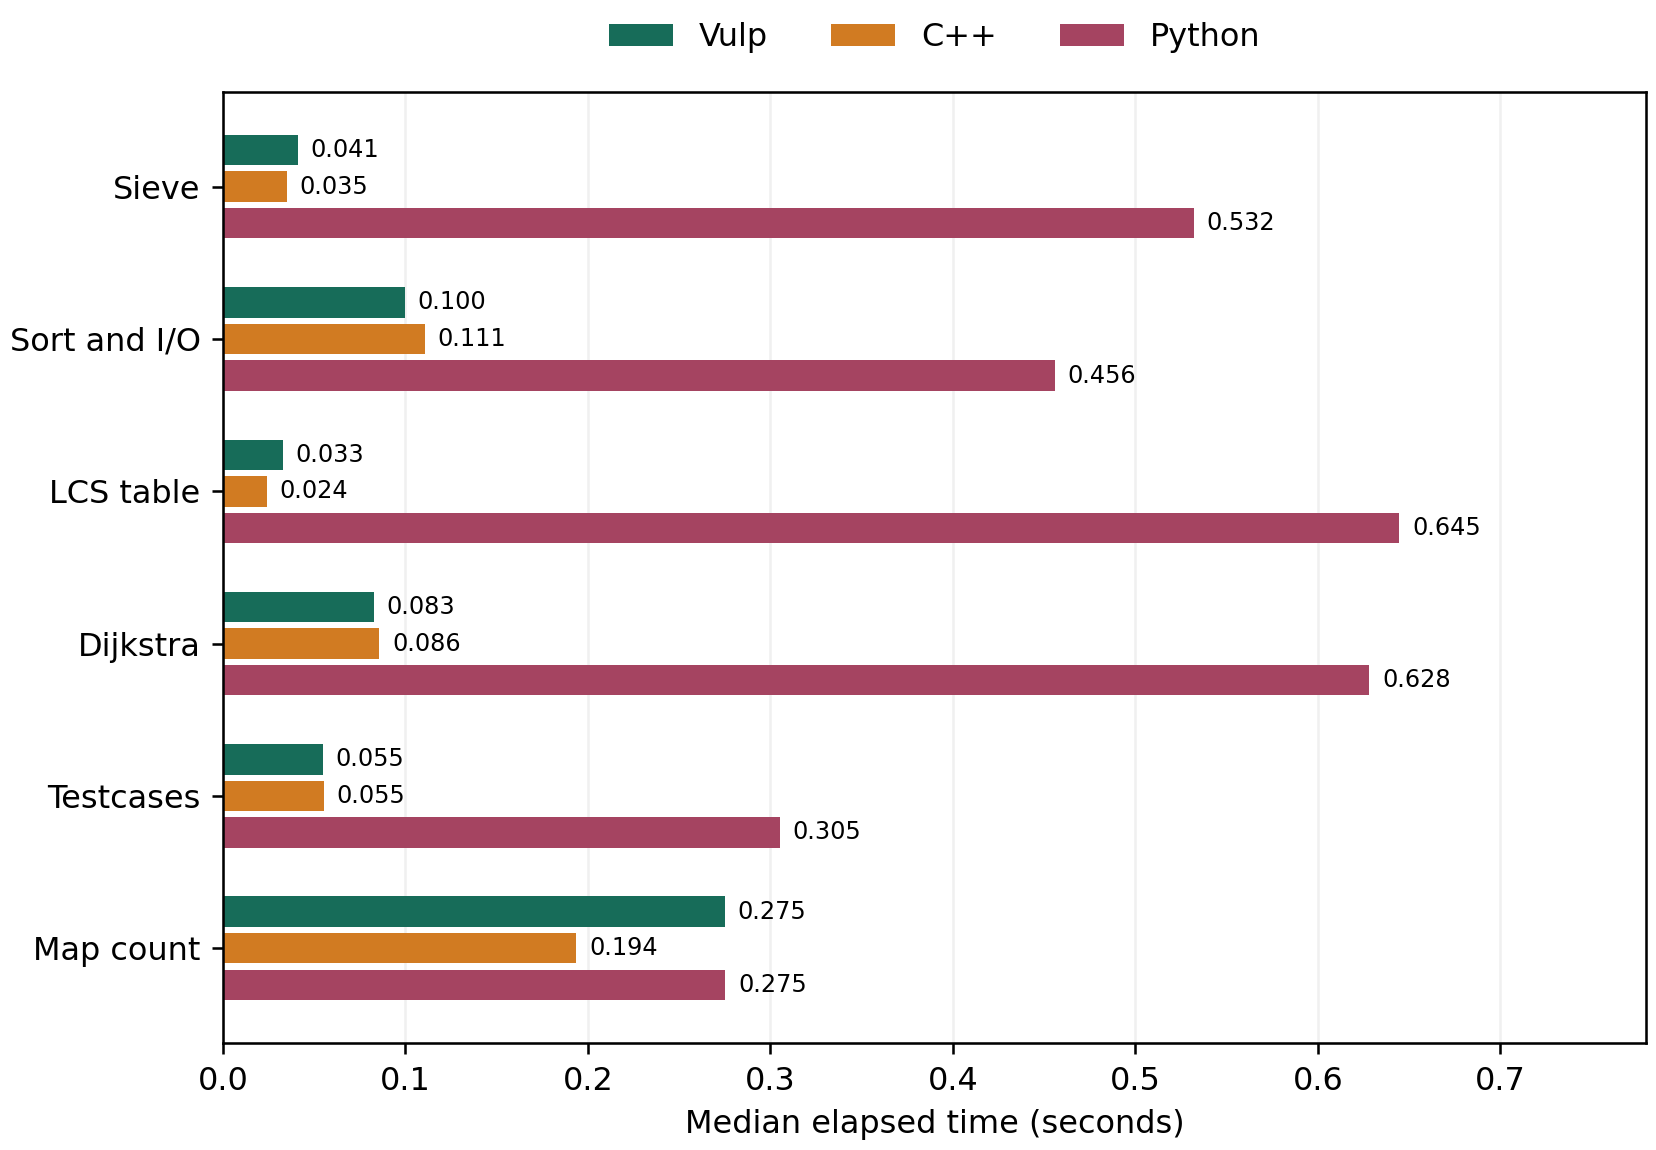
\includegraphics[width=0.97\textwidth]{laptop_runtime.png}
\caption{Median elapsed time in seconds for each implementation. The linear horizontal scale starts at zero; lower is better. LCS uses 32-bit table elements in \vulp{} and C++.}
\label{fig:laptop-runtime}
\end{figure}

Four \vulp{} programs finish within 17\% of the C++ time. Map counting is slower: the runtime allocates values separately and makes an extra key lookup during iteration. The checked \vulp{} LCS table, with \texttt{i32} elements, takes 0.033 s and 38.1 MiB. The C++ table also has 32-bit elements and takes 0.024 s and 37.5 MiB. The measured \vulp{} time is therefore 1.37 times the C++ time for this task.

The container representation affects memory use too. Map counting reaches 22.8 MiB in \vulp{} and 15.5 MiB in C++; Dijkstra reaches 21.4 MiB and 21.0 MiB. For sorting and I/O, Python reaches 188.1 MiB while \vulp{} reaches 11.4 MiB. These values are peak resident memory for the entire process, including runtime overhead.

\section{Source size and build time}
We counted the source tokens for the same six programs in Table~\ref{tab:tokens} and Figure~\ref{fig:source-tokens}. Five \vulp{} solutions use fewer tokens than their C++ counterparts. Dijkstra goes the other way because V1 lacks a priority queue and its \vulp{} source includes a handwritten binary heap. Token count gives one reproducible measure of source length. It does not measure the time spent writing or debugging.

\begin{table}[htbp]
\centering\small
\begin{tabular}{|l|r|r|r|}
\hline
Task & Vulp tokens & C++ tokens & Token reduction\\\hline
Sieve & 83 & 143 & $42\%$\\\hline
Sort and I/O & 22 & 118 & $81\%$\\\hline
LCS, i32 table & 138 & 196 & $30\%$\\\hline
Dijkstra & 518 & 344 & $-51\%$ \\\hline
Testcases & 59 & 134 & $56\%$\\\hline
Map count & 86 & 146 & $41\%$\\\hline
\end{tabular}
\caption{Source-token counts for the six tasks. Dijkstra includes a handwritten heap in Vulp because V1 has no priority queue.}
\label{tab:tokens}
\end{table}

\begin{figure}[htbp]
\centering
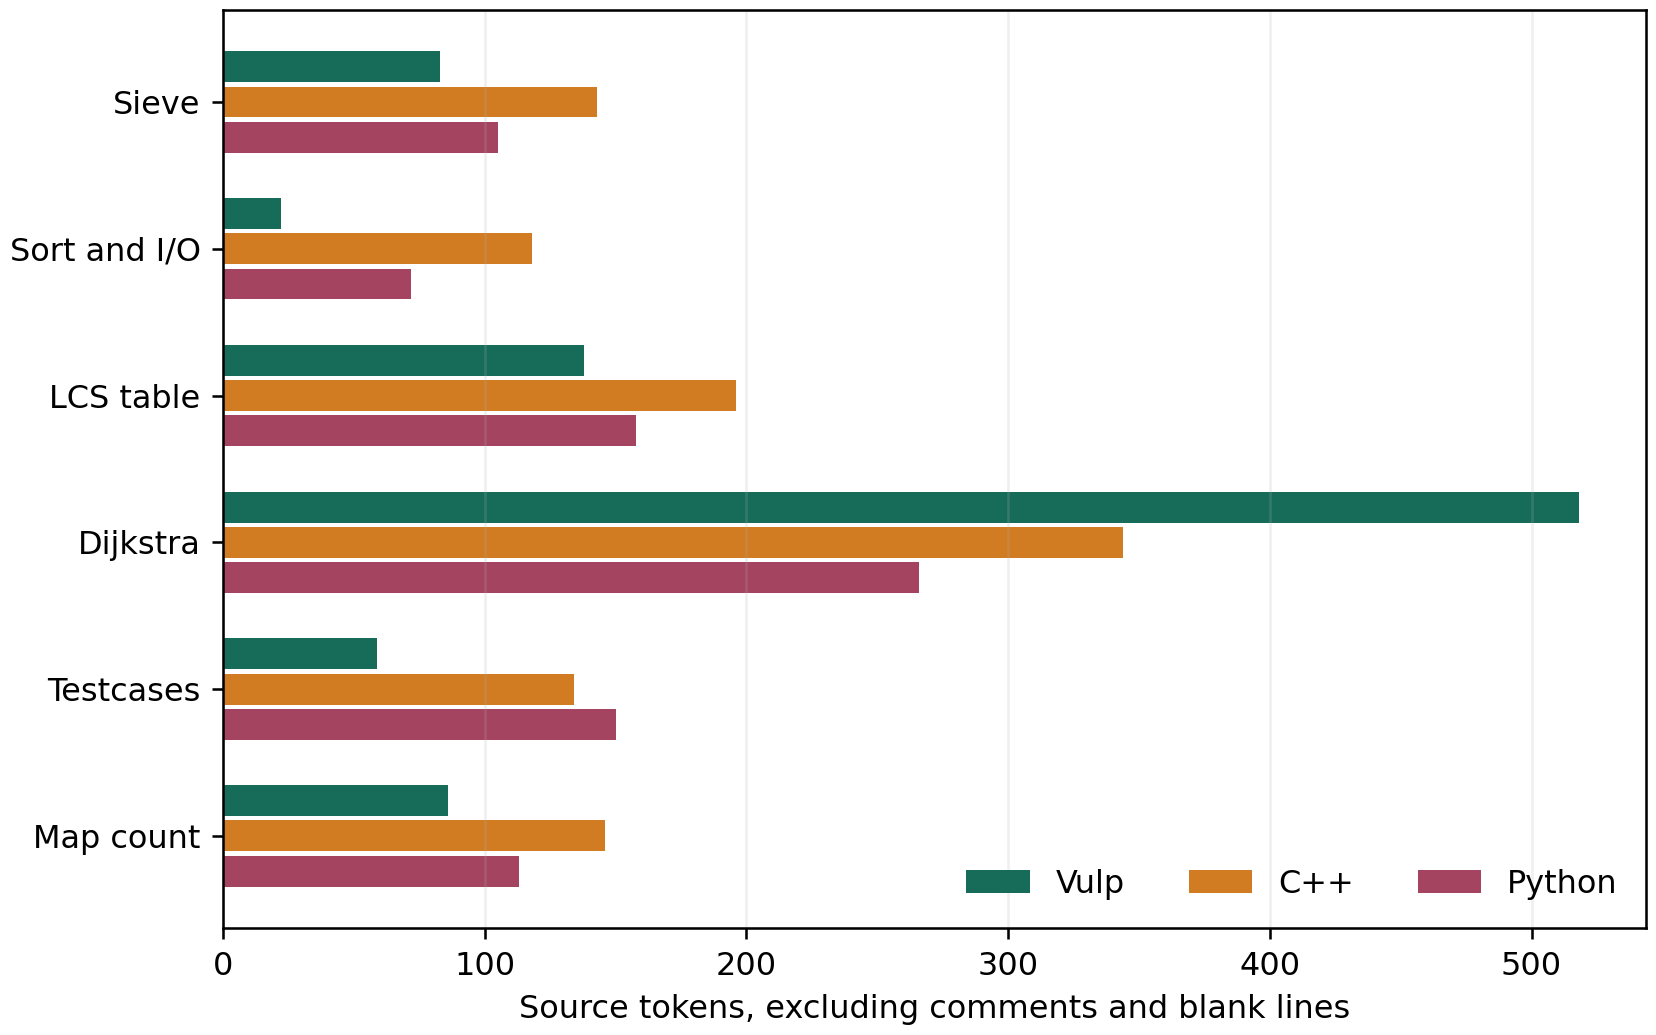
\includegraphics[width=0.97\textwidth]{source_tokens.png}
\caption{Source-token counts for the six task implementations. All three languages solve the same input-output task in each row.}
\label{fig:source-tokens}
\end{figure}

For these six programs, \texttt{vulpc} takes about 0.05 to 0.06 s to build a native executable. The C++ builds take about 0.96 to 1.05 s. They include \texttt{<bits/stdc++.h>}, so the result would differ with a smaller or precompiled header. The runtime table uses prebuilt executables, although \vulp{} programs can also be run through the JIT while testing.

\clearpage
\section{Representative source comparisons}
The next two examples show the full programs used for sorting and sieving in each language. We removed comments and blank lines for display and wrapped long expressions to fit the columns. The token counts come from the original files, after excluding comments and blank lines. The time and memory values come from the seven-round measurements in Table~\ref{tab:existing-time}.

\subsection{Sorting one million integers}
Each program reads $n$ integers and prints them in ascending order on one line. The \vulp{} program reads directly into a sized array, calls \texttt{sort}, and prints the array with \texttt{println}.

\noindent\begin{minipage}[t]{0.315\textwidth}
\small\textbf{Vulp}\par\hrule\scriptsize
\begin{verbatim}
read int n;
read int[n] a;
a.sort();
println(a);
\end{verbatim}
\end{minipage}\hfill
\begin{minipage}[t]{0.315\textwidth}
\small\textbf{C++}\par\hrule\scriptsize
\begin{verbatim}
#include <bits/stdc++.h>
using namespace std;
int main() {
  ios::sync_with_stdio(false);
  cin.tie(nullptr);
  int n;
  cin >> n;
  vector<long long> a(n);
  for (auto& x : a) cin >> x;
  sort(a.begin(), a.end());
  for (int i = 0; i < n; i++)
    cout << a[i]
         << (i + 1 < n
             ? ' ' : '\n');
}
\end{verbatim}
\end{minipage}\hfill
\begin{minipage}[t]{0.315\textwidth}
\small\textbf{Python}\par\hrule\scriptsize
\begin{verbatim}
import sys
def main():
    data = (sys.stdin.buffer
            .read().split())
    n = int(data[0])
    a = sorted(map(
        int, data[1:n + 1]))
    sys.stdout.write(
        " ".join(map(str, a))
        + "\n")
main()
\end{verbatim}
\end{minipage}

\begin{center}\small
\begin{tabular}{|l|r|r|r|}
\hline
Measure & Vulp & C++ & Python\\\hline
Median elapsed time (s) & 0.100 & 0.111 & 0.456\\\hline
Peak resident memory (MiB) & 11.4 & 10.8 & 188.1\\\hline
Source tokens & 22 & 118 & 72\\\hline
\end{tabular}
\end{center}
\noindent The \vulp{} program uses 81\% fewer source tokens than C++. Its time and peak memory are close to the C++ values. Python uses much more memory because this program reads and splits the whole input at once.

\clearpage
\subsection{Sieve of Eratosthenes}
Each program counts primes through $n=2\times10^7$ and prints the count and largest prime. All three mark composite numbers. Python performs its inner marking step with a byte-array slice assignment, so its work is organized differently from the loops in the compiled programs.

\noindent\begin{minipage}[t]{0.315\textwidth}
\small\textbf{Vulp}\par\hrule\scriptsize
\begin{verbatim}
read int n;
bool[n + 1] composite;
int count = 0, last = 0;
for i in [2..n]: {
  if composite[i]: continue;
  count++;
  last = i;
  for (int j = i * i;
       j <= n; j += i):
    composite[j] = true;
}
println(count, " ", last);
\end{verbatim}
\end{minipage}\hfill
\begin{minipage}[t]{0.315\textwidth}
\small\textbf{C++}\par\hrule\scriptsize
\begin{verbatim}
#include <bits/stdc++.h>
using namespace std;
int main() {
  ios::sync_with_stdio(false);
  cin.tie(nullptr);
  long long n;
  cin >> n;
  vector<char> composite(n + 1);
  long long count = 0, last = 0;
  for (long long i = 2;
       i <= n; i++) {
    if (composite[i]) continue;
    count++;
    last = i;
    for (long long j = i * i;
         j <= n; j += i)
      composite[j] = 1;
  }
  cout << count << " " << last
       << "\n";
}
\end{verbatim}
\end{minipage}\hfill
\begin{minipage}[t]{0.315\textwidth}
\small\textbf{Python}\par\hrule\scriptsize
\begin{verbatim}
import sys
def main():
    n = int(
        sys.stdin.buffer
        .readline())
    composite = bytearray(n + 1)
    count = last = 0
    for i in range(2, n + 1):
        if composite[i]:
            continue
        count += 1
        last = i
        if i * i <= n:
            composite[
                i * i::i] = (
                b"\x01" *
                len(range(
                    i * i,
                    n + 1, i)))
    print(count, last)
main()
\end{verbatim}
\end{minipage}

\begin{center}\small
\begin{tabular}{|l|r|r|r|}
\hline
Measure & Vulp & C++ & Python\\\hline
Median elapsed time (s) & 0.041 & 0.035 & 0.532\\\hline
Peak resident memory (MiB) & 22.9 & 22.3 & 48.1\\\hline
Source tokens & 83 & 143 & 105\\\hline
\end{tabular}
\end{center}
\noindent Here \vulp{} uses 42\% fewer tokens than C++. The compiled programs have similar peak memory: \vulp{} takes 0.041 s and C++ takes 0.035 s. The Python version shown above takes 0.532 s.

\section{Memoization against direct recursion}
LCS has nine million states arranged in a dense table. Generic memoized recursion is expensive for that workload, so we also tested a recurrence where repeated calls are the main cost: Fibonacci. The plain \vulp{}, C++, and Python functions evaluate the same recurrence without a memo table. The memoized \vulp{} function differs only in its \texttt{dp fn} declaration. We checked every output against the expected Fibonacci number before accepting its timing. The programs, measurement script, and raw runs are in \texttt{vulp/docs/report/bench/dp\_fib/}.

We compiled \vulp{} and C++ with \texttt{-O2} and used Python 3.12.3. Each run started a fresh process, read $n$ from standard input, and computed the answer. We used three interleaved rounds for each of $n=34$, 37, and 40 on the reference laptop. The table reports the median wall time, including process startup and Python interpreter startup. The \texttt{dp fn} values are close to the process-startup floor, so they are not measurements of individual calls.

\noindent\begin{minipage}{\linewidth}
At $n=40$, plain recursion takes about 126 times as long as \texttt{dp fn} in \vulp{}, 68 times as long in C++, and 5267 times as long in Python. These ratios have a small denominator because \texttt{dp fn} finishes near process-startup time. Ordinary Fibonacci recursion revisits arguments many times; the memoized version computes the 41 distinct inputs from 0 to 40 once each. Plain C++ is faster than plain \vulp{} in this experiment. The useful feature of \texttt{dp fn} is that it adds caching without a manually written table.
\end{minipage}

\begin{table}[htbp]
\centering\small
\begin{tabular}{|r|r|r|r|r|}
\hline
$n$ & Vulp \texttt{dp fn} & Vulp plain & C++ plain & Python plain\\\hline
34 & 0.001498 & 0.012353 & 0.006476 & 0.465477\\\hline
37 & 0.001324 & 0.048304 & 0.029392 & 1.943468\\\hline
40 & 0.001568 & 0.197658 & 0.106929 & 8.259869\\\hline
\end{tabular}
\caption{Fibonacci experiment: median elapsed seconds, three rounds, fresh process for each run. All programs produced the same integer.}
\label{tab:fib}
\end{table}

\begin{figure}[htbp]
\centering
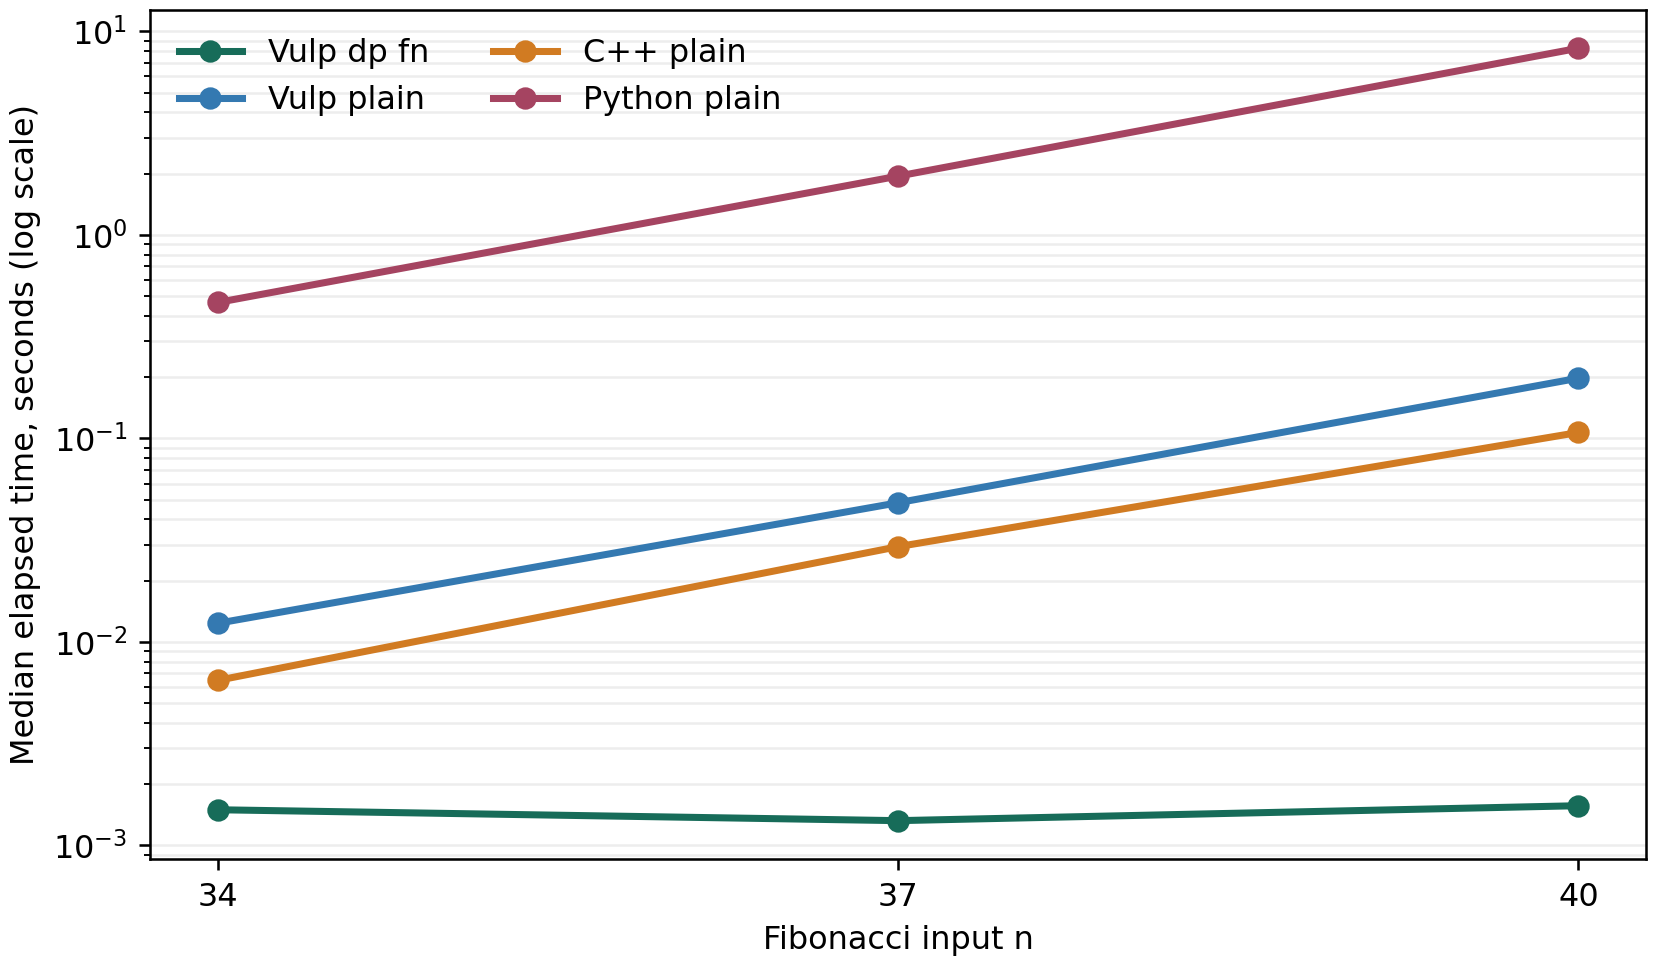
\includegraphics[width=0.97\textwidth]{fib_runtime.png}
\caption{Median elapsed time in seconds for the same Fibonacci recurrence. The logarithmic scale shows growth in unmemoized recursion and nearly constant observed time for \texttt{dp fn} over these inputs.}
\label{fig:fib-runtime}
\end{figure}

\begin{figure}[htbp]
\centering
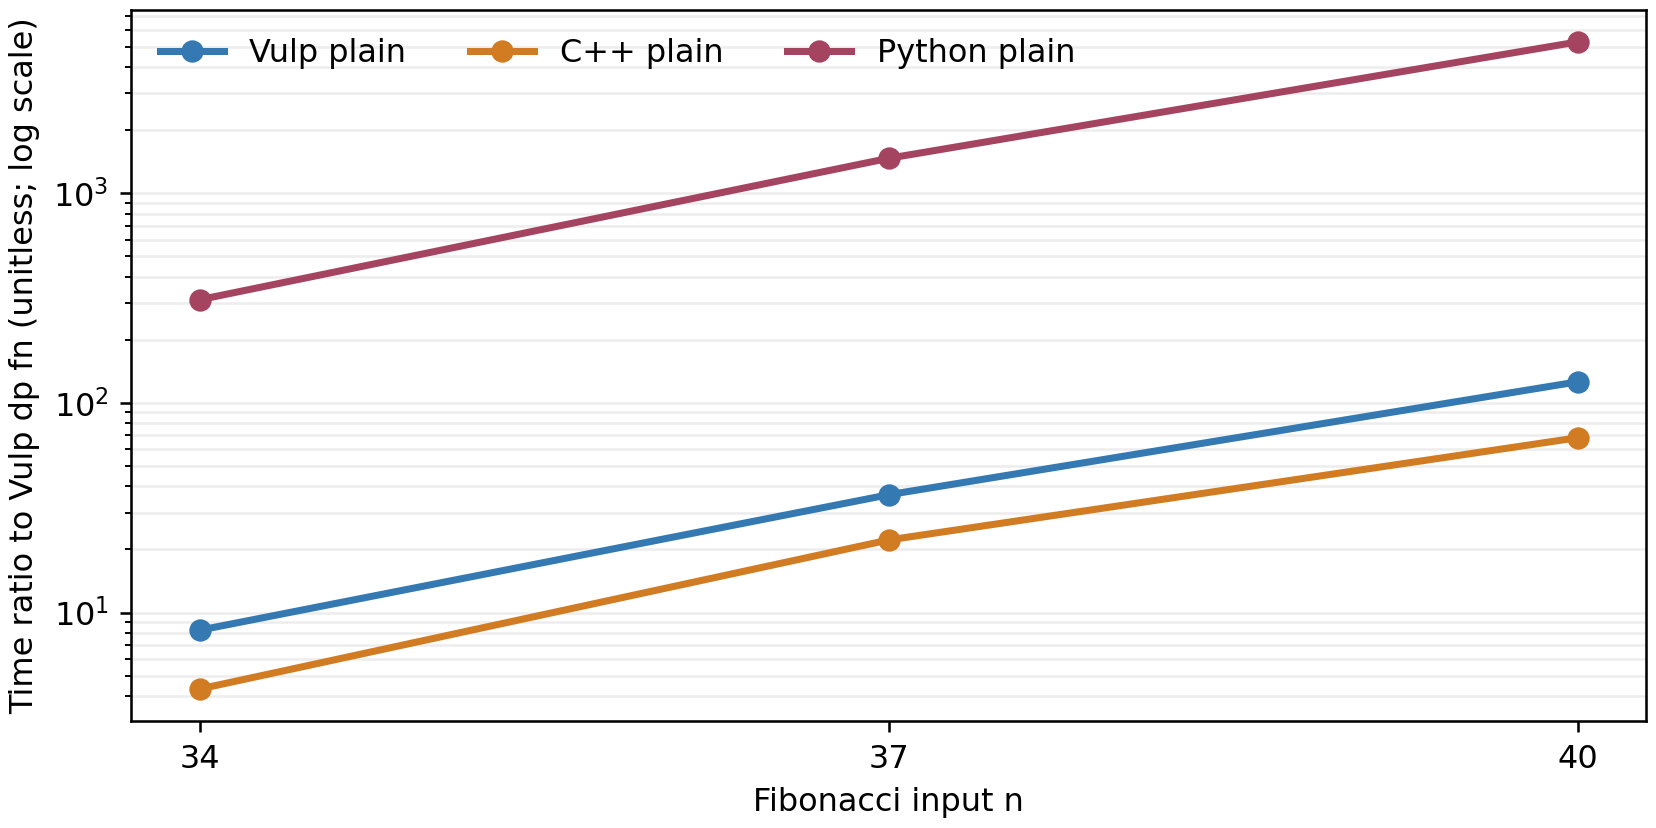
\includegraphics[width=0.97\textwidth]{fib_speedup.png}
\caption{Plain-recursion time divided by \texttt{dp fn} time at each input size. This ratio is unitless; the underlying elapsed times include process startup.}
\label{fig:fib-speedup}
\end{figure}

\clearpage
\section{Limits of the evidence}
Fibonacci has extensive repeated recursion, which makes it a good test for memoization. It is a poor basis for predicting every dynamic program. On LCS, a dense problem, the \vulp{} \texttt{dp fn} program takes 1.581 s and 675.7 MiB. The checked \texttt{i32} table takes 0.033 s and 38.1 MiB. Caching removes repeated calls, but the table uses a more suitable representation for this set of states. We have also yet to measure C or Java programs and the time people spend writing solutions.

\chapter{Progress against the proposal}\label{ch:progress}
Our initial proposal calls for a CP-specific IR, data-structure selection, string algorithms, and complexity analysis in addition to the compiler. Table~\ref{tab:progress} shows where each item stands at this review. \texttt{PROGRESS\_CHECKLIST.md} gives a more detailed checklist.

\small
\begin{longtable}{|>{\raggedright\arraybackslash}p{41mm}|>{\raggedright\arraybackslash}p{24mm}|>{\raggedright\arraybackslash}p{63mm}|}
\caption{Status of proposal goals at Phase 1 Review 2.}\label{tab:progress}\\
\hline
Proposal item & Status & Implemented result or next step\\\hline
\endfirsthead
\hline Proposal item & Status & Implemented result or next step\\\hline
\endhead
Custom lexer, parser, type checking & Implemented & Source under \texttt{src/lexer}, \texttt{src/parser}, and \texttt{src/sema}; unit tests cover each stage.\\\hline
LLVM IR and native compiler & Implemented & \texttt{src/codegen} and driver support JIT and object emission.\\\hline
Fast input and testcase syntax & Implemented & Buffered runtime I/O and \texttt{TC:} examples.\\\hline
Exact-width and range-declared integers & Partial & Widths to 256 bits are supported; declared range limits are not enforced at run time.\\\hline
Automatic DP memoization & Implemented & \texttt{dp fn} with purity checks and testcase cache reset.\\\hline
CP-specific IR and range-query selection & Planned & No \texttt{range\_q} selection among prefix, Fenwick, segment, and sparse-table forms.\\\hline
DP layout selection & Planned & Dense arrays exist; compiler-directed rolling rows, sparse storage, and bitset layouts do not.\\\hline
Graph abstraction and layout selection & Planned & Adjacency structures can be programmed with vectors; no built-in graph or CSR selection.\\\hline
Modular arithmetic type and bitset & Planned & Neither proposed abstraction is present as a built-in type.\\\hline
String algorithms and first-class functions & Planned & Strings and ordinary functions exist; rolling hash, KMP, Z-function, and function values are absent.\\\hline
Time and memory complexity annotations & Planned & No static complexity-contract syntax or verifier is present.\\\hline
Optional small language model & Exploratory & No AI mode exists in the compiler; it must remain separate from verified static results.\\\hline
C, C++, Java, Python benchmark & Partial & Six-task suite measures C++ and Python; Fibonacci study adds direct recursion baselines.\\\hline
40 to 50 contest problems and writing-effort study & Planned & Current measured suite has six task families and no user study.\\\hline
\end{longtable}
\normalsize

\section{Next implementation steps}
We plan to start with a representation for range queries that records exactly which updates and queries the program makes. Static sums could then use a prefix array; point additions with prefix sums could use a Fenwick tree; and other supported operations could call for a segment tree. The compiler's choice should be visible to the programmer and tested against simple reference implementations.

For dynamic programming, we need dependence information before the compiler can replace a full table with rolling rows. That transformation is valid only when the recurrence no longer uses the older rows. We will also test bitsets on boolean or small-alphabet problems. Modular arithmetic and graph APIs need defined semantics and runtime measurements before we choose their final form.

Complexity annotations will need a restricted syntax and a way to distinguish proved bounds from unresolved cases. If we explore a small language model, its output will be labelled as an estimate and checked against static evidence where possible. It cannot stand in for a proof. We also plan to add C and Java baselines, more complete contest problems, peak-memory and compilation-time measurements, and a controlled exercise measuring writing effort.

\chapter{Conclusion}
We have built a working LLVM-based compiler for \vulp{} with a custom frontend, native and JIT execution, buffered input, testcase syntax, wide integers, containers, and checked memoization. In the six measured tasks, several \vulp{} programs run close to C++ while using fewer source tokens. The map and LCS results also show costs that the compiler still needs to address. In Fibonacci, adding \texttt{dp fn} avoids repeated recursion without requiring a hand-written cache; in dense LCS, a table is much more efficient.

The proposed data-structure selection and complexity contracts are still to be implemented. Our next phase will test those features on more contest problems and compare compiler-selected representations with ones chosen by hand.

\begin{thebibliography}{99}
\addcontentsline{toc}{chapter}{References}
\bibitem{atcoder} AtCoder, ``AC Library Documentation,'' \url{https://atcoder.github.io/ac-library/production/document_en/}.
\bibitem{kactl} KTH Algorithm Competition Template Library, project repository, \url{https://github.com/kth-competitive-programming/kactl}.
\bibitem{llvmref} LLVM Project, ``LLVM Language Reference Manual,'' \url{https://llvm.org/docs/LangRef.html}.
\bibitem{llvmtutorial} LLVM Project, ``My First Language Frontend with LLVM,'' \url{https://llvm.org/docs/tutorial/MyFirstLanguageFrontend/}.
\bibitem{graphit} Y. Zhang et al., ``GraphIt: A High-Performance DSL for Graph Analytics,'' \emph{Proceedings of the ACM on Programming Languages}, vol. 2, OOPSLA, article 121, 2018. \url{https://doi.org/10.1145/3276491}.
\bibitem{nanz} S. Nanz and C. A. Furia, ``A Comparative Study of Programming Languages in Rosetta Code,'' \emph{Proceedings of ICSE}, pp. 778--788, 2015. \url{https://doi.org/10.1109/ICSE.2015.90}.
\bibitem{knoth} T. Knoth et al., ``Liquid Resource Types,'' 2020. \url{https://arxiv.org/abs/2006.16233}.
\end{thebibliography}
\end{document}
